\usetikzlibrary{arrows.meta,
                chains,
                positioning,
                quotes,
                shapes.geometric}

\tikzset{FlowChart/.style={% this style can be used also at other flowcharts,
                           % just call it with "FlowChart", see picture code below
startstop/.style = {rectangle, rounded corners, draw, fill=red!30,
                    minimum width=3cm, minimum height=1cm, align=center,
                    on chain, join=by arrow},
  process/.style = {rectangle, draw, fill=orange!30,
                    text width=5cm, minimum height=1cm, align=center,
                    on chain, join=by arrow},
 decision/.style = {diamond, aspect=1.5, draw, fill=green!30,
                    minimum width=3cm, minimum height=1cm, align=center,
                    on chain, join=by arrow},
       io/.style = {trapezium, trapezium stretches body,   % not used in your flowchart
                    trapezium left angle=70, trapezium right angle=110,
                    draw, fill=blue!30,
                    minimum width=3cm, minimum height=1cm,
                    text width =\pgfkeysvalueof{/pgf/minimum width}-2*\pgfkeysvalueof{/pgf/inner xsep},
                    align=center,
                    on chain, join=by arrow},
    arrow/.style = {thick,-Triangle}
                        }
        }% end of tikzset
% --------------------------------------------------------------
\begin{chapter}{Global Sensitivity Analysis for Stochastic Simulators\label{Ch:sensitivity}}
\section{Introduction}
A simulator used to make statements about a real-world system needs realistic parameter settings. Some parameter values have little uncertainty about them. It is well understood that, close to the earth's surface, acceleration due to gravity takes the value $g = 9.81ms^{-2}$. For complex engineering projects implementing new technologies, the values parameters should take may not be well understood.

In the wind farm setting, consider the lifetime of a gearbox. We may have some understanding of the gearbox lifetime from laboratory testing, such as step accelerated life testing \citep{Nelson1980}. This testing will have been performed under laboratory conditions which offer an imperfect replication of real-world conditions. Although the test will provide a useful indication of the lifetime of a gearbox, there will be marked differences between the test environment and real-world conditions. Alternatively, we may be using old technologies in new environments, and so there will exist historical data from which quantities of interest can be inferred under a different set of conditions to the planned use case. For example, we may be employing onshore technology in an offshore environment, or pushing offshore technology much further away from the shore into deeper waters. In either case, we may have a good understanding of how the technology works in a limited range of conditions. There are intricacies to every problem which need to be considered; for example, the location of the wind farm will have an impact on gearbox lifetimes. Components used in an onshore wind farm in a mild climate will likely last considerably longer than those used in a harsh, offshore environment. This problem can be expressed as trying to obtain the conditional probability $P(T < t \mid E )$ where $T$ is the lifetime of a component such as a gearbox. The event $E$ denotes all relevant aspects of the wind farm, such as the wind farm topology and details of its location. Since there will never have previously been a wind farm with properties described by $E$, the probability $P(T < t \mid E)$ is difficult to obtain with data. A practical solution to this problem is to elicit probability distributions from experts for uncertain quantities \citep{Syed2020, Wilson2021, Dalal2022}.

This input uncertainty means that, even for deterministic computer simulations, the output is also uncertain. Let us return to the gearbox example. Suppose one aspect of $E$ is that the wind farm will be in operation for $20$ years. If the lifetime distribution was specified, or estimated, to be $T \mid E \sim \mathcal{N}(40, 5^2)$, then it is reasonable to assume that gearbox lifetime will have negligible impact on wind farm performance. Whereas if the lifetime distribution is given by $T \mid E \sim \mathcal{N}(10, 3^2)$, it is likely that many gearboxes will fail during the operation of the wind farm and thus gearbox performance could have serious implications for availability. When there are many uncertain parameters in a black-box simulator, it is not clear which are the main contributors to output uncertainty. In the context of eliciting parameters for a complex simulator this is important. Probability elicitation is a time intensive task; especially when multiple experts are used \citep{Williams2021}. Although elicitation is a time consuming task, it is typically much faster and cheaper than collecting an equivalent sample of data.

If an input is deemed important in the simulator, we should elicit the probability distribution over this parameter carefully. We should consider details such as the shape of the parameter's probability distribution. Less important parameters can be assigned a distribution less rigorously; for example a Normal distribution with an appropriate mean or mode (possibly truncating the distribution to avoid non-physical values) or a uniform distribution with appropriate limits. The least important parameters can be assigned a point mass at a plausible value, or be assigned simple distributions. This essentially follows the SHELF guidelines of spending the most time on the most important parameters; see the ``Many Quantities of Interest'' document from \citet{SHELF4} for an elaboration on this philosophy. An illustration of how an elicitation for forward uncertainty propagation can be assisted by emulators and sensitivity analysis is given in \Cref{Fig:elicitation-flowchart}. The first emulator will typically be constructed with all relevant unknowns in mind, whereas the emulator constructed in light of refined uncertainty may be a simpler emulator. In particular, it may be appropriate to construct the emulator over only the more important variables and either condition on a plausible value for unimportant parameters or, if unimportant variables are varied in an experiment, they can be accounted for via the nugget term.
\begin{figure}

\begin{center}
\resizebox{0.4\textwidth}{!}{
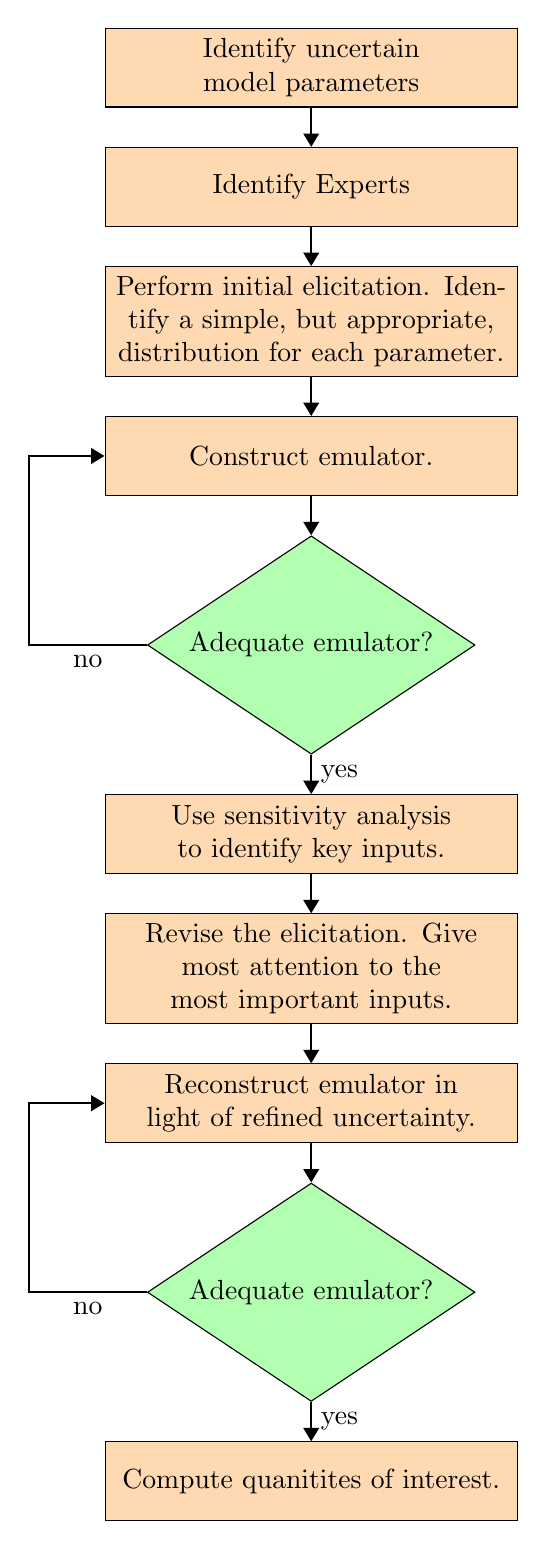
\begin{tikzpicture}[FlowChart,                   % used are styles from tikzset FlowChart
    node distance = 5mm and 7mm,
      start chain = A going below                    % The nodes in the chain
                                                     % will be named by A-1, A-2, ...
                        ]
\node   [process] {Identify uncertain model parameters};               % A-1
\node   [process]   {Identify Experts}; %A-2
\node   [process]   {Perform initial elicitation. Identify a simple, but appropriate, distribution for each parameter.};%A-3
\node   [process]   {Construct emulator.};%A-4
\node   [decision] {Adequate emulator?};%A-5
\node   [process]   {Use sensitivity analysis to identify key inputs.};%A-6
\node   [process]   {Revise the elicitation. Give most attention to the most important inputs.};%A-7
\node   [process]   {Reconstruct emulator in light of refined uncertainty.};%A-8
\node   [decision] {Adequate emulator?};%A-9
\node   [process]   {Compute quanitites of interest.};%A-10
% lines not considered by join macro
\draw [arrow] (A-5.west) to ["no"] ++ (-1.5,0) |- (A-4);
\path   (A-5) to ["yes"] (A-6);
\draw [arrow] (A-9.west) to ["no"] ++ (-1.5,0) |- (A-8);
\path   (A-9) to ["yes"] (A-10);
    \end{tikzpicture}
}
\end{center}

\caption{Illustration of how emulators and sensitivity analysis can be used to assist the elicitation for forward uncertainty propagation.}
\label{Fig:elicitation-flowchart}
\end{figure}

The above discussion is well characterised by the following three questions about output uncertainty induced by input uncertainty in a complex simulator:
\begin{itemize}
    \item[1.] If $\bx$ is uncertain; what is the associated uncertainty about $y(\bx)$?
    \item[2.] If $\bx$ is a vector of uncertain inputs, which elements of $\bx$ are contributing the most uncertainty to $y(\bx)$?
    \item[3.] If $y(\cdot)$ is a stochastic simulator, how much output uncertainty is coming from the inherent stochasticity of $y(\cdot)$? How much output uncertainty stems from uncertainty about $\bx$?
\end{itemize}

We will now briefly review some approaches to understanding the impact of uncertain inputs to a simulation model.

\section{Approaches to understanding input uncertainty}

\subsection{Scenario analysis}

A basic approach to considering the impact of input uncertainty is a scenario analysis \citep{Zhang2012, Grewal2013}. The goal of scenario analysis is to make statements of the form \textit{``If we assume $\bx$ happens then $y(\bx)$ will happen''}.

A scenario analysis takes a finite collection of inputs $\mathcal{X}_0 = \{ \bx_1, \bx_2, \ldots, \bx_n\}$  and compares their outputs; $y(\bx_1)$, $y(\bx_2)$, \ldots, $y(\bx_n)$. The set $\mathcal{X}_0$ might be chosen as the sets of inputs corresponding to a desirable scenario, an undesirable scenario and an intermediate scenario. $\mathcal{X}_0$ may also be chosen as a set of moderate inputs and some extreme inputs. If $y(\cdot)$ is stochastic the analyst would analyse the distribution generated by each $\bx_i$. A discussion of scenario analysis is given by \citet{Wheatcroft2019}; they provide details of choosing $\mathcal{X}_0$.

One criticism of this approach is that it is not very exploratory. Scenario analysis only considers a small number of values of $\bx$ and thus we gain a limited understanding of how $\bx$ impacts $y(\bx)$. Even for input vectors of moderate dimension (say $4$), examining the outputs of just a handful of input configurations gives virtually no knowledge of the underlying behaviour of $y(\bx)$.

Another criticism of this approach is that it does not consider how likely each scenario, and hence each $\bx_i$, is; if $y(\bx_1)$ suggests that the wind farm is destined to fail but an expert assessed that $\bx_1$ has negligible density, we might not worry too much about the implications of this scenario.

Although scenario analysis is not well suited to constructed a detailed understanding of complex simulations, it does serve a role in understanding broad, less well defined questions \citep{Criqui2012, Samso2020}.

\subsection{OAT analysis}
One-at-a-time (OAT) analysis aims to generate understanding of $y(\bx)$ (or $f(\bx)$) by varying only the $i$th inputs, $x_i$ over some pre-specified range whilst keeping the remaining inputs, $\bx_{-i}$, fixed at some nominal values. Plotting $f(x_i \mid \bx_{-i})$ allows us to study the influence of $x_i$ on $f(\bx)$ or $y(\bx)$. This type of analysis is very popular outside of the statistical community \citep{Holvoet2005,Khalid2016, Saraiva2017}. OAT analysis is attractive since it is conceptually simple. In varying just one input at a time, we can easily see how $x_i$ impacts the simulator output. There is no noise introduced by varying additional variables (unless $y(\cdot)$ is stochastic). However, a very simple example shows a shortcoming in fixing $\bx_{-i}$ at some nominal value. We argue that this is a naive approach to understanding input importance via the following example.

Consider the following simulator
\begin{equation}
f(x_1, x_2) = x_1 x_2. \label{Eq:oat-simulator}
\end{equation}
\Cref{Eq:oat-simulator} is overly-simplistic and known, but we will imagine it is a black-box. Suppose a modeller conducts an OAT analysis and they choose to vary $x_1$ and $x_2$ over the range $(-1,  1)$. The analyst may then vary $x_1$ over this range whilst fixing $x_2 = 0$, the midpoint of the range. Since $f(x_1, 0) = 0$ for any $x_1$ it appears that $x_1$ has no impact whatsoever on $f(\cdot)$. No simulator of practical interest will be as simple as this, but  \cref{Eq:oat-simulator} displays an important flaw in OAT analysis: an OAT analysis \textit{cannot} detect interactions. Another important criticism of OAT is that, asymptotically, it is a local sensitivity analysis \citep{Saltelli2010}. The argument is constructed by considering the volume of the input space explored compared to the total volume of the input space. Suppose that $\bx \in [0,1]^m$. If we vary inputs individually, we only explore points within the $m$ dimensional hypersphere of radius $\frac{1}{2}$, rather the full hypercube of input configurations. The relative volume of the hypersphere of radius $\frac{1}{2}$ to the unit hypercube is
\begin{equation}
  RV(m) = \frac{\pi^{\frac{m}{2}}}{2^m \Gamma\left(1 + \frac{m}{2}\right)}.
\end{equation}
This expression is fairly complex but, by observing that $\frac{\sqrt{\pi}}{2} < 0.9$ we see that
\begin{equation}
  RV(m) < \frac{0.9^m}{ \Gamma \left(1 + \frac{m}{2}\right) } \to 0 \text{ as } m \to \infty
\end{equation}
since $0.9^m$ is a monotonically decreasing function of $m$, and $\Gamma(1 + \frac{m}{2})$ is monotonically increasing when $m \in [1, \infty)$. The effects of this asymptotic result are felt at small $m$, thus the idea that OAT analysis is `global' is a bit of a myth. For a $9$ dimensional input configuration, like our Athena example from the previous chapter, $RV(9) = 0.0064$. Thus if we were to perform an OAT analysis, we would be exploring less that $1\%$ of the parameter space. $RV(m)$ is plotted in \cref{Fig:relative-volume}. This plot illustrates that, even for problems of small-to-moderate dimension, an OAT analysis is severely under-exploring the input space.  This leads to poor inferences about $f(\cdot)$.
\begin{figure}
  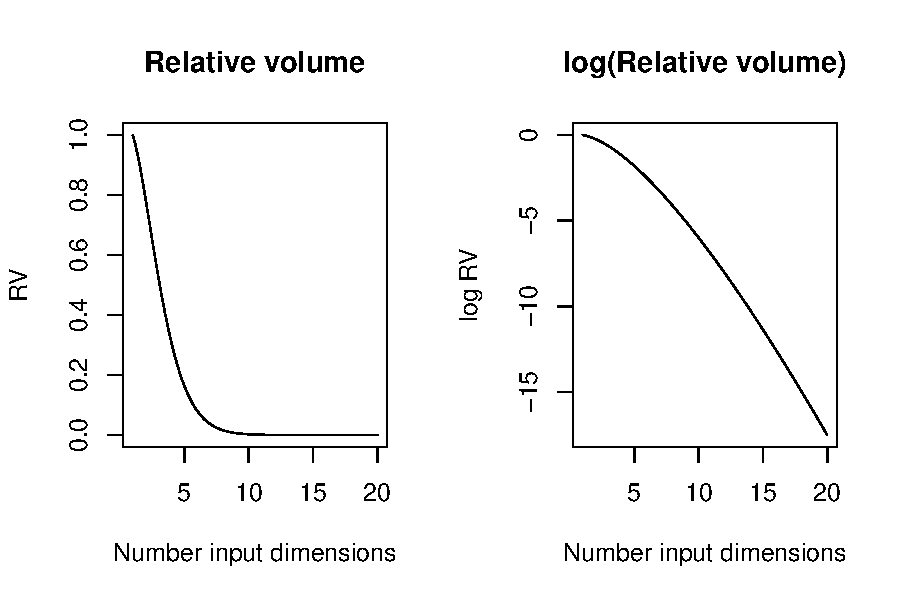
\includegraphics{fig-sensitivity/relative-volume.pdf}
  \caption{Plots showing $RV(m)$ (left) and $\log RV(m)$ (right) for $1 \leq m \leq 20$. Once $m  \geq 10$ the relative volume is essentially $0$. \label{Fig:relative-volume}}
\end{figure}
To consider the full hypercube of input configurations (or a more general shape when inputs are constrained \citep{Kucherenko2017, Kotidis2019}) we need to perform integration. One integration based method is probabilistic sensitivity analysis (PSA). This is frequently called variance based sensitivity analysis and we use the terms interchangeably.
\section{Probabilistic sensitivity analysis for deterministic simulators}
\subsection{Some notation}
Throughout the remainder of this chapter, we will be working with the expectation and variance with respect to
\begin{itemize}
  \item[(i)]  $G(\bx)$ -- the distribution characterising uncertainty about simulator inputs, $\bx$.
  \item[(ii)] $\pi(y(\cdot) \mid \mathcal{D})$ and $\pi(f(\cdot) \mid \mathcal{D})$ -- the posterior distribution of simulator output for stochastic and deterministic simulators respectively.
  \item[(iii)] When $y(\cdot)$ is a stochastic simulator, it will have its own expectation, $\E \{ y(\cdot) \} = f(\cdot) $ and variance $\var \{ y(\cdot) \} = \lambda^2(\cdot)$.
\end{itemize}
To avoid confusion between the expectation and variance induced by $G(\bx)$ and the expectation and variance induced by $\pi(y(\cdot) \mid \mathcal{D})$, we will use $\E_\bx$ and $\var_\bx$ to denote moments with respect to $G(\bx)$. Moments with a $*$ superscript ($\E^{*}$, $\var^{*}$) denote the moments of posterior distributions of simulator outputs. In other words, with respect to $\pi(y(\cdot) \mid \mathcal{D})$ or $\pi(f(\cdot) \mid \mathcal{D})$. We will retain the $m^{*}$  and $v^{*}$ notation used in previous chapters when referring to the posterior mean and variance of $y(\cdot)$. We will use operators without a subscript ($\E$ and $\var$) to denote the ``true'' moments of $y(\cdot)$ and $\log \lambda (\cdot)$.

This section relies on sampling many collections of inputs, $\bx \sim G(\bx)$. We also condition on elements of $\bx$ on many occasions. We will use subscripts, $x_i$, $\bx_J$, to denote elements and sub-vectors of $\bx$. When drawing values of $\bx$ from a (joint) distribution, we will use the notation $\bx^{(j)}$ to denote the $j$th sample of $\bx$.

\subsection{Probabilistic sensitivity analysis}
Within the statistical community, PSA is the go-to method for global sensitivity analysis for two reasons:
\begin{itemize}
  \item[1.] PSA is a global method.
  \item[2.] The output of PSA is straightforward to interpret.
\end{itemize}
One output of PSA is a collection of sensitivity indices (sometimes called Sobol' indices) representing the proportion of uncertainty induced on simulator output by collections of uncertain inputs. The main drawback is that probabilistic sensitivity analysis can be computationally expensive. Thousands of simulator runs are required to obtain reliable estimates of quantities of interest.

When emulators are used in place of a deterministic simulator, $f(\cdot)$, the computational cost is manageable \cite{Becker2012, Overstall2016}. With emulator assisted probabilistic sensitivity analysis, the majority of the computational budget is spent on training an appropriate emulator, which will typically be of the order of a few hundred runs of the simulator. This may be more expensive than a scenario or OAT analysis, but allows for full parameter space exploration and inference about interactions of any order between inputs.

PSA proceeds by specifying a distribution over the inputs $G(\bx)$ and propagating this distribution, and various conditional distributions based on $G(\bx)$, through $f(\bx)$. Sensitivity indices tell us what proportion of the variance in the model output, $V = \var(Y)$, where $Y = f(\bx)$ is the uncertain simulator output, is induced by the uncertainty in (subsets of) inputs $\bx$. First we consider sensitivity analysis for a deterministic simulator and then extend this to the stochastic setting.
\begin{comment}
In the context of probability elicitation, PSA is the go-to method for determining input importance. \citet{Ohagan2012} presented elicitation as a $6$ stage process. In stages $1$--$3$ no probability judgements are elicited. Initial probability judgements are elicited in the $4$th stage. The $5$th stage is revision of beliefs. In this stage, the facilitator shows the experts consequences of their judgements and challenges their beliefs. If this distribution is not compatible with the beliefs of the experts, this suggests that the initial specification should be revised. When a complex simulator is involved, it is usually the case that a small subset of inputs are driving the variability in simulator output(s) \citep{Kennedy2006, Vernon14}. Since the simulator is complex, it is unclear which inputs are driving the outputs. The Sheffield Elicitation Framework (SHELF) approach to expert elicitation advises the elicitation facilitator to spend the largest amount of resources (time and money are two such resources) on the most important parameters. \citet{Ohagan2012} is interested in eliciting parameters of a complex computer model and goes on to perform PSA to determine input importance. The distribution used in the PSA is one obtained from the 4$th$ stage of elicitation. The facilitator should then use the results of PSA to guide stage $5$. In particular, pay most attention to the most
\end{comment}
\subsection{The functional ANOVA decomposition}
PSA relies on the functional ANOVA decomposition. If $\bx$ is a $m$-dimensional input vector then the functional ANOVA decomposition of a function $f(\bx)$ is
\begin{equation}
 f(\bx) = f_0 + \sum_i f_i(x_i) + \sum_{i < j} f_{i,j}(\bx_{i,j}) + \sum_{i<j<k} f_{i,j}(\bx_{i,j,k}) + \ldots + f_{1, 2, \dots, m}(\bx) \label{Eq:functional-anova}
\end{equation}
which is unique when $\bx$ has probabilistically independent components. In \cref{Eq:functional-anova}, $f_0 = \E_\bx(Y)$, and
\begin{equation}
    f_i(x_i) = \E_{\bx_{-i}} (Y \mid x_i ) - f_0
\end{equation}
is the main effect of $x_i$ on $f(\bx)$. The first order interaction effect of $x_i$ and $x_j$ (where $i<j$) is
\begin{equation}
    f_{i,j}(\bx_{i,j}) = \E_{\bx_{-(i,j)}} (Y \mid x_i, x_j ) - f_i(x_i) - f_j(x_j) - f_0.
\end{equation}
This is the effect due to \textit{only} the interaction between $x_i$ and $x_j$, as their main effects are subtracted. Higher order effects for some non-empty subset $J$ of $\{1, 2, \ldots, m\}$ can be extracted from the functional ANOVA decomposition by finding $\E_{\bx_{-J}} (Y \mid \bx_{J} )$ and then subtracting relevant interaction and main effect terms. Plotting $f_i(x_i)$ allows us to understand how $x_i$ influences $f(\bx)$. Likewise, plotting first order effects allows us to understand how pairs of inputs influence $f(\bx)$. This is similar to an OAT analysis but allows for interaction terms and averages over $\bx_{-i}$, rather than conditioning on a single value.
\subsection{Sensitivity indices}
Main effect and interaction plots allow us to gain an intuition of how influential $\bx_J$ is on $f(\bx)$. It is often useful to assign an interpretable value to the relative influence of $\bx_i$ on $f(\bx)$. In PSA, this is achieved by considering the variance of \cref{Eq:functional-anova}.

If $G(\bx) = \prod_i G_i(x_i)$ then taking the variance of both sides of \cref{Eq:functional-anova} leads to
\begin{align}
 \var(Y) &= \sum_{J \subseteq \{1, 2, \ldots, m\} }  \var_{\bx_{J}} \{ f_J(\bx_J) \}\\
         &= \sum_{J \subseteq \{1, 2, \ldots, m\} }  \var_{\bx_{J}}  \{ \E_{\bx_{-J}} [ Y \mid \bx_J ] \}
\end{align}
The above sum has $2^{m} - 1$ terms; one for each non-empty subset of $\{1, 2, \ldots, m \}$.
The first type of sensitivity index is
\begin{align}
    S_i &= \frac{V_i}{V}\\
    V_i & = \var_{x_{i}} \{ \E_{\bx_{-i}} [ y(\bx) \mid X_{i} ] \}.
\end{align}
Here, $S_i$ is the proportion of $\var\{Y\}$ induced by the uncertainty about $x_i$. This tells us that, if we were to learn the `true' value of $x_i$, then we would expect $\var\{Y\}$ to decrease by $100S_i\%$. This can be generalised to any subset $J$;
\begin{equation}
 S_J = \frac{1}{V} \sum_{J' \subseteq J} V_{J'}
\end{equation}
\correction{where $S_J$ is the amount of variability explained by the variables corresponding to $J$.}

The second type of sensitivity index is
\begin{equation}
    S_{T_i} = \frac{V - \var_{x_{-i}} \{ \E_{x_i} (Y \mid \bx_{-i}) \} }{V}
\end{equation}
which represents the proportion of $\var_\bx \{Y\}$ remaining when all inputs apart from $x_i$ have been learnt. \correction{This can be generalised to $S_{T_J}$, which represents the remaining uncertainty when all inputs apart from those corresponding to $J$ have been learnt.} In this chapter we focus mainly on $S_J$ rather than $S_{T_J}$ since we are interested in using sensitivity analysis for probability elicitation. We need to deduce how to reduce uncertainty about $\bx$ in a way which efficiently reduces uncertainty about $Y$, which is what $S_i$ tells us. The $S_i$ and $S_J$ have a natural decision theoretic justification as measures of importance, which we now discuss.
\subsection{Linking PSA to EVPI: decision theoretic justification for $S_i$}
Let $u(a, \bx)$ be a utility function for decision $a \in \mathcal{A}$ when the (random) consequence $\bx$ occurred. Let $U(a) = \E_\bx \{ u(a, \bx) \} $ be the expected utility of decision $a$. Let $U^* = U(a^*)$ where $a^* = \argmax_{a \in \mathcal{A}} U(a)$ is the optimal decision.

In decision theory, EVPI (expected value of perfect information) is the price the decision maker would pay to obtain the precise value of an uncertain quantity $x_i$. The EVPI for input $i$ is given by
\begin{equation}
    \text{EVPI}_i = \E_{x_i} \left\{  \max_{a \in \mathcal{A}} \E_{\bx \mid x_i} u(a, \bx)  \right\} - U^*.
\end{equation}
EVPI is interpreted as the price a decision maker would pay to have access to perfect information; the true value of $x_i$. In our context, `perfect information' is the true value of an uncertain parameter to a simulator. Now suppose our goal is to obtain the true value, or the best possible point estimate, of $f(\bx)$ when $\bx$ itself is uncertain. To define the `best possible' point estimate, a Bayesian would specify a utility function describing how (un)desirable using $a$ as an estimate of $f(\bx)$ is. A commonly used utility function in estimation routines is squared loss. Thus we take our utility function to be
\begin{align}
U(a) &= -\E_{\bx} \{(a - f(\bx))^2\}\\
      &= -a^2 + 2a\E_{\bx} \{ f(\bx) \} + \E_{\bx} \{ f(\bx)^2 \}
\end{align}
which is maximised at $a^{*} = \E_{\bx} \{ f(\bx) \} $, the expected simulator output. Thus the EVPI, under this utility function is,
\begin{align}
\text{EVPI}_i &= \E_{x_i} \{ -\var_{X_{-i}}[ f(\bx) \mid X_i ]  \} - (-)\var_\bx \{ f(\bx) \} \\
              &= \var_{\bx} \{ f(\bx) \} -\E_{X_i} \{ \var_{\bx_{-i}}[ f(\bx) \mid x_i ] \}\\
              &= \var_{x_i} \{ \E_{\bx_{-i}} [ f(\bx) \mid x_i ]  \}\\
              &= V_i.
\end{align}
The sensitivity index $S_i = V_i / V$ improves the interpretability of EVPI; $S_i$ represents the proportion of variation in $f(\bx)$ explained by $x_i$. This relationship between $S_i$ and EVPI tells us that, if $S_k$ is the largest sensitivity index and we are able to learn the precise value of only one input, then we should learn $x_k$. If we can learn two inputs, then we should learn the pair $(k, l)$ which maximise $S_k + S_l + S_{k,l}$. If we want to learn $Q$ inputs, we should learn the set $J$ of size $Q$ which maximises $\sum_{J' \subseteq J} S_J'$.

\subsection{Computation of sensitivity indices}

\citet{Sobol1993} provides Monte Carlo based algorithms for computing sensitivity indices. Many runs are required to compute the indices, which is not problematic for computationally cheap simulators. Slow run times of complex simulators induce a computational bottleneck in PSA. Replacing the simulator by an emulator provides huge computational savings without much loss of accuracy when the simulator is computationally expensive. In the deterministic case, particular forms of $G(\bx)$ lead to a tractable emulator-based PSA \citep{Oakley04}. We will present the more general case via Monte Carlo simulation, which does not rely on the form of emulator or specification of $G(\bx)$. The Monte Carlo case also allows for distributional estimates of $S_J$, whereas \citet{Oakley04} produce only $\E^{*}\{V_J\}$ and $\var^{*}\{V_J\}$.
\subsubsection{Constructing main effects plots}
To begin the analysis we must estimate $f_0$. This is achieved via the usual estimate of the mean;
\begin{align}
f_0 & = \int f(\bx) \,\dd G(\bx) \\
& \approx \frac{1}{N} \sum_{j = 1}^N f (\bx^{(j)}) \\
& =  \hat{f}_0
\end{align}
where $\bx^{(j)} \iid G(\bx)$. Simple i.i.d. sampling returns an \correction{unbiased} estimate for $f_0$. If each $x_i \sim U(a, b)$ then Latin Hypercube sampling offers an estimate that is still unbiased but more efficient \citep{Mckay1979, Stein1987}.

Estimates of main effects are given by
\begin{align}
f_i(x_i) &  = \int f(\bx) \,\dd G(\bx_{-i} \mid x_i ) - f_0\\
	& \approx \frac{1}{N} \sum_{j = 1}^N f(\bx^{(j)} \mid x_i)  - \hat{f}_0. \label{Eq:main-effect-est}
\end{align}
Now, $f_i(x_i)$ is a function; plots of $f_i(x_i)$ are constructed by evaluating \cref{Eq:main-effect-est} over a sequence of values for $x_i$.

Estimation of the functions implied by interaction effects is as follows:
\begin{equation}
\hat{f}_{i,j}(x_{i,j}) = \frac{1}{N} \sum_{k = 1}^N f(\bx^{(k)} \mid x_{i,j})  - \hat{f}_i(x_i) - \hat{f}_j(x_j) - \hat{f}_0. \label{Eq:interaction-plot-est}
\end{equation}

The above estimation procedures assume that we are directly using the simulator. If we are using a GP emulator to facilitate computation then we have posterior distributions for these quantities. The posterior mean of $\hat{f}_i(x_i)$ is obtained by replacing $f(\bx)$ by $m^*(\bx)$ in \cref{Eq:main-effect-est} and \cref{Eq:interaction-plot-est}. The posterior variance can be found by replacing $f(\bx)$ by $v^{*}(\bx)$, and turning subtractions into additions. Monte Carlo estimates can be obtained by drawing random functions from $\pi(f(\cdot) \mid \mathcal{D})$  to produce a probability distribution for $f(x_i)$.

\subsubsection{Estimating sensitivity indices}

To estimate $V$, assuming direct use of the simulator, we can use the standard variance estimate;
\begin{equation}
 \hat{V} = \frac{1}{N-1} \sum_{j=1}^N (f(\bx^{(j)}) - f_0)^2.
\end{equation}

To compute $V_i$ we need to find the variance of an expectation. Some manipulation of expectations gives us a more attractive way forward. Starting from the definition of $V_i$ we have
\begin{align}
V_i &= \var_{x_i} \left\{  \E_{\bx_{-i}} [f(\bx)\mid x_i] \right\}\\
    &= \E_{x_i}\left\{  \E_{\bx_{-i}} [f(\bx)\mid x_i]^2 \right\} - \E_{x_i}\left\{  \E_{\bx_{-i}} [f(\bx)\mid x_i] \right\}^2\\
    &= \E_{x_i}\left\{  \E_{\bx_{-i}} [f(\bx)\mid x_i]^2 \right\} - \E_{\bx} \{ f(\bx) \}^2.
\end{align}
Now a Monte Carlo estimate of $E_{\bx} \{ f(\bx) \}^2$ is straight forward; $(\hat{f}_0)^2$. This will be slightly biased for $\E_{\bx}\{f(\bx)\}^2$, but with sufficiently large $N$, the bias will be negligible. The use of an emulator means obtaining sufficiently large $N$ is not a problem. Estimating $T_i  = \E_{x_i}\left\{  \E_{\bx_{-i}} [f(\bx)\mid x_i]^2 \right\}$ is a bit more of a challenge. An efficient estimation method --- under the assumption that $\bx$ is uniformly distributed on $[0, 1]^m$ is given in Chapter $8$ of \citet{Gramacy2020surrogates}. \correction{We illustrate this algorithm in \cref{alg:est-Si} under the assumption that $G_i(x_i) = \mathcal{U}(0, 1)$.}

\begin{algorithm}[h]
\caption{Point estimation of $S_i$}\label{alg:est-Si}
\begin{algorithmic}
\Require Estimates $\hat{f}_0 \approx \E_\bx \{ f(\bx) \} $, $\hat{V} \approx \var_{\bx} \{ f(\bx) \}$.
\For{$i = 1$, $2$, $\ldots$, $m$}
  \State Construct an $N \times m$  Latin hypercube, $X$
  \State \correction{$\tilde{X} \gets X$}
  \For{$j = 1$, $2$, $\ldots$, $N$}
  \State $\tilde{x}_{i,j} \sim G_i(x_i)$ \Comment{Re-draw the $i$th elements of $\tilde{\bx}_j$}
  \EndFor
  \State $\hat{T}_i \gets \frac{1}{N-1}\sum_{j=1}^N m^{*}(\bx_j)m^{*}(\tilde{\bx}_j)$
  \State $\hat{S}_i \gets \frac{\hat{T}_i - \hat{f}^2_0}{\hat{V}}$
\EndFor
\State Return estimated sensitivity indices $\hat{S}_1$, $\hat{S}_2$, \ldots, $\hat{S}_m$.
\end{algorithmic}
\end{algorithm}
Bayesian estimation is based on having many posterior draws of $f(\cdot)$. If draws are available, then for each draw we execute \cref{alg:est-Si} and return the set of point estimates as a single draw of each value. Many draws are used to approximate the joint posterior distribution of the $S_i$.

It is straightforward to adapt \cref{alg:est-Si} can be adapted to when $\bx$ is not uniformly distributed on $[0,1]^m$ but does have probabilistically independent elements. We replace $G_i(x_i)$ by the distribution of $x_i$ and the $i$th column of $X$ must be $N$ i.i.d. samples from $G_i(x_i)$, this column must also be independent of the other columns.

\correction{The above MC estimates are often relying on one or more previously found MC estimates. The convergence of these `nested' MC schemes (NMC) has been analysed in the machine learning literature. For example, \citet{Rainforth2018} provide optimal convergence rates for NMC schemes. In general, convergence is slower as the number of nested approximations increases. In this work, we only have two levels of nesting (the variance of the mean), and our emulators are sufficiently cheap that achieving negligible bias with a small wall-clock CPU time is achievable.}

\section{Extending PSA to the stochastic case}
The Athena simulator is stochastic so the illustrated methodology needs to be adapted. Re-applying the above methodology to the emulator mean will allow us to perform inference about $\E\{ y(\cdot) \}$. Because the illustrated approach was devised with deterministic simulators in mind it cannot address two important aspects of sensitivity analysis in stochastic simulation:
\begin{itemize}
	\item[1.] Quantifying the amount of output uncertainty induced by the stochastic nature of the simulator.
	\item[2.] Understanding which input variables are driving the stochasticity.
\end{itemize}
Fortunately, \citet{Marrel2012} present an appropriate solution to both the above concerns which places few restrictions on the form of the emulator.  The core requirements are a model for the mean and another for the variance (or other measure of dispersion). Therefore, their approach applies to our HetGP and SML emulators constructed in \cref{Ch:Hetsml}. They compartmentalise the simulator; $y_m(\bx) = \E \{ y(\bx) \} $ is the mean component of the simulator and $\lambda^2(\bx) = y_d(\bx) = \var \{ y(\bx) \} $ is the dispersion component. We will retain our notation from \cref{Ch:Hetsml} using $f(\cdot)$ and $\lambda^2(\cdot)$  to denote the `true' mean and variance of $y(\cdot)$. The approach of \citet{Marrel2012} formulates a stochastic computer model $y(\cdot)$ as a function of $\bx$, the simulator inputs, but also $x_\varepsilon$, the state of the pseudo random number generator of the simulator. Although, in theory, we could `open up' the black box simulation and observe the state of the random number generator, we treat $x_\varepsilon$ as an unknown quantity. We refer to $x_\varepsilon \in \N$ as the ``seed variable''.
\subsection{Determining input importance for $y(\bx)$}
Since $f(\bx) = \E \{ y(\bx) \}$ is a deterministic function, the ANOVA decomposition is precisely the same as \cref{Eq:functional-anova}. In addition, $y(\bx)$ has a similar functional ANOVA decomposition which takes $x_\varepsilon$ into consideration
\begin{equation}
y(\bx) = f(\bx) + f_\varepsilon(\bx) + \sum_{J \subseteq \{1, 2, \ldots, m\}} f_{\varepsilon, J}(\bx) \label{Eq:stoch-anova}
\end{equation}
where $f_\varepsilon(\bx)$ is the main effect of the seed variable and $f_{\varepsilon, J}(\bx)$ represents the interaction term between the seed variable and the subset of variables attributed to the set $J$. As with the deterministic case, $V_J/V$, determines how much uncertainty of the subset of variables $J \subseteq \{1, 2, \ldots, m \}$ contributes to the total variance in $y(\bx)$. However, because $y(\bx)$ is stochastic, the total variance formula tells us that
\begin{align}
V & = \var_{\bx} \{ \E[y(\bx) \mid \bx ] \} + \E_{\bx} \{ \var[y(\bx) \mid \bx] \}\\
  &  = \var_\bx \{ f(\bx) \} + \E_\bx \{ \lambda^2(\bx) \}.
\end{align}
The definition of $V$ has been adjusted to account for stochasticity, therefore,
\begin{equation}
\sum_{J \subseteq \{1, 2, \ldots, m \} } V_J < V.
\end{equation}
The additional variability comes from $x_\varepsilon$. We now have
\begin{equation}
V = \left( \sum_{J \subseteq \{1, 2, \ldots, m \} } V_J \right)+ V_{T_{\varepsilon}}
\end{equation}
with $V_{T_{\varepsilon}}  = V \times S_{T_\varepsilon}$ being the total variance induced by $x_\varepsilon$.
\subsection{Determining input importance for $\log \lambda^2(\bx)$}
Under the HetGP and SML assumptions, $\log \lambda^2(\bx)$ is an arbitrary function. To avoid cumbersome notation, we define $\ell(\bx) = \log \lambda^2 (\bx)$. A functional ANOVA decomposition of $\ell(\bx)$ is also possible. We adopt the convention used in \cref{Ch:Hetsml} and place a $\lambda$ superscript on any quantities related to $\ell(\bx)$. The functional ANOVA decomposition of $\ell(\bx)$ is
\begin{equation}
\ell(\bx) = f^{\lambda}_0 + f^{\lambda}_\varepsilon (\bx) + \sum_{J\subseteq \{ 1, 2, \ldots, m\}} f^{\lambda}_J(\bx) . \label{Eq:lambda-anova}
\end{equation}
There are no interaction terms between $\bx$ and $x_\varepsilon$ in \cref{Eq:lambda-anova} because  $\lambda^2_V$ is assumed constant. It would be possible to construct an ANOVA decomposition of the variance of $\ell(\bx)$, however, this is a fourth order statistic. Emulation of this quantity is discouraged since estimates of fourth order statistics can be highly unstable and it is not clear what the benefits of such an analysis would be \citep{Andrianakis2017}.
Sensitivity indices for $\log \lambda^2(\bx)$ proceed in a similar way to $y(\bx)$. The total variance of $\ell(\bx)$ is given by
\begin{equation}
\var_\bx \{ \ell(\bx)\} = \lambda^2_V + \var_{\bx} \{\correction{ \E [ \ell(\bx) ] }  \}
\end{equation}
where \correction{$\E \{ \ell(\bx) \} $} is the `true' value of $\ell (\bx)$. The $S^{\lambda}_J$ have definitions which follow naturally from $S_J$ and and $S_{T_\varepsilon}$. In the log variance context, $S^{\lambda}_{T_\varepsilon}$ is the amount of uncertainty about $\log \lambda^2(\bx)$ that is present due to the stochasticity of simulations. We can also compute main effects in an analogous way to $y(\bx)$.
\subsection{Computation of sensitivity indices}
We discuss some details of the computation of the sensitivity indices in the stochastic case as well as understanding the importance of $S_{T_\varepsilon}$. We only provide details of point estimates of the quantities of interest; however our results later give posterior distributions for the sensitivity indices. The posterior distributions are obtained by drawing random functions from the emulator and computing a corresponding point estimate for each draw.
Computation of $S_{T_\varepsilon}$ is fairly simple. First we need to estimate $V$. To do this, we use
\begin{equation}
\hat{V} = \widehat{\var}_{\bx} \{ f(\bx) \}  + \bar{\lambda}^2 (\bx)
\end{equation}
where
\begin{align}
\bar{\lambda}^2 (\bx) &  = \frac{1}{N} \sum_{j=1}^N \hat{\lambda}^2(\bx)\\
\widehat{\var}_{\bx} \{ f(\bx) \} \ &= \frac{1}{N-1} \sum_{j=1}^N (m^*(\bx^{(j)}) - \hat{f}_0)^2
\end{align}
and then
\begin{equation}
 \hat{S}_{T_\varepsilon} = \frac{\hat{V} - \widehat{\var}_{\bx} \{ y_m(\bx) \} }{\hat{V}}. \label{eq:steps-hat}
\end{equation}
Introduction of $S_{T_\varepsilon}$ is one of the novel contributions from \citet{Marrel2012}; it is the total proportion of variability attributed to the stochastic nature of $y(\cdot)$. The physical interpretation of $S_{T_\varepsilon}$ is the total sensitivity attributed to all stochastic processes in the simulator. It essentially measures how random a simulator is.
Then estimates of $S_i$ follow directly from estimates of $T_i$, $\E_\bx \{y(\bx) \}$ and $V$ and have the usual interpretation. \citet{Marrel2012} suggest estimating $S_{T_\varepsilon}$ by \cref{eq:steps-hat} to ensure that $S_{T_\varepsilon} + \sum S_J = 1$. We cannot compute $S_\varepsilon$ or any $S_{\varepsilon, J}$; they are non-identifiable because $x_\varepsilon$ is not observed. Thus we have a limited understanding of how important the stochasticity in the simulator is or how the seed interacts with elements of $\bx$.

\section{Application of PSA to the Athena simulator}
We apply the above methodology to the Athena simulator. To facilitate the computation, we use our SML emulator from \cref{Ch:Hetsml} which emulated $\probit \left[ A(\bx) \right]$ for a $9$ dimensional, uncertain input vector $\bx$. The elements of $\bx$ are exactly the same as in the previous chapter. As a reminder, they are the mean time to failure for the 9 sub-assemblies; 1. gearbox, 2. generator, 3. frequency converter (freq. conv.), 4. transformer, 5. main shaft bearing (MSB), 6. blades, 7. tower, 8. foundations, and 9. catch all.

We also revisit the HetGP emulator. We know that the SML emulator improved RMSE and score. The black-box nature of emulators means it is difficult to see \textit{why} one emulator offers a better representation of the simulator. Since main effect plots give an impression of the shape of the simulator we may be able to understand why one emulator has outperformed the other. The results here are also presented in \citet{Kennedy2023}.

Our choice of $G(\bx)$ is given by $x_i \iid \mathcal{U}(0.1, 5)$, which is uniform over the range of inputs our emulators were constructed. This is a useful and practical distribution for PSA when we have limited access to experts \citep{Saisana2005,Overstall2016}. Our estimation approach is Bayesian; we draw $1000$ different functions from the posterior distribution and then for each draw compute Sobol' sensitivity indices based on Latin hypercube samples of size $N=10^4$. Boxplots of first order indices based on both HetGP and SML are given in \Cref{Fig:si-mean}. In both cases, $\sum_{i=1}^9S_i + S_{T_\varepsilon}\approx 1$ suggesting Athena is approximately additive in the inputs. Some realisations of $S_i$ are negative, this is a symptom of Monte Carlo error and happens when $S_i \approx 0$ \citep{Gramacy2020surrogates}. Note that all posterior means and medians of $S_i$ are positive, and the negative draws are usually identified as outliers, indicated by a $\times$ on the boxplots.
\begin{figure}[ht]
   \centering
   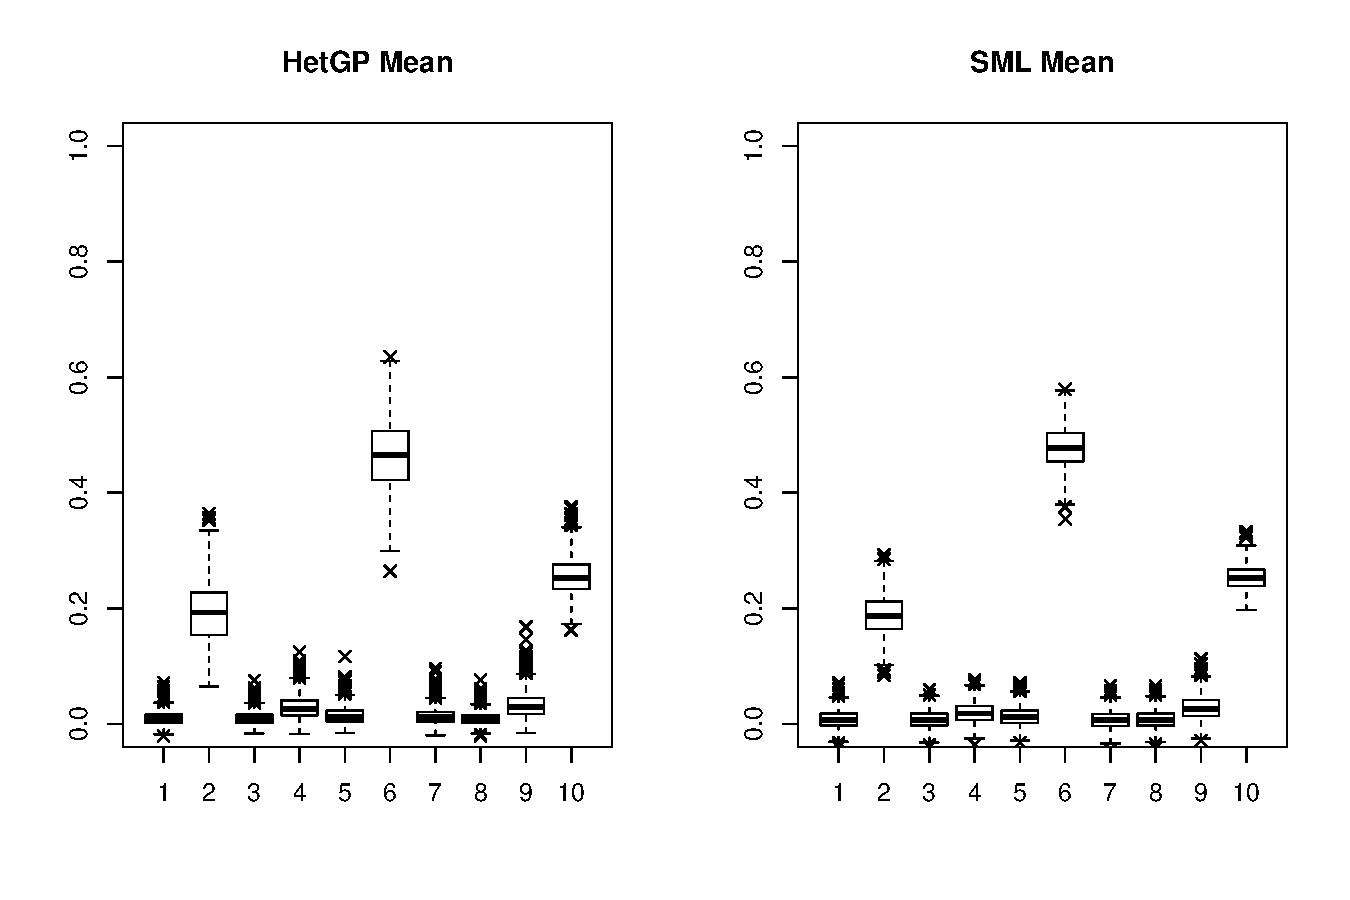
\includegraphics[width=0.9\textwidth]{fig-sensitivity/si-mean4.pdf}
   \caption{Boxplots representing the posterior distribution of $S_i$; $i=1$, $2$, \ldots, $9$. The $10^{th}$ index corresponds to $S_{T_\varepsilon}$. The left hand plot corresponds to HetGP; the right hand to SML.}  \label{Fig:si-mean}
\end{figure}
We should not worry about small differences amongst the $S_i$ since they are functionals of $G(\bx)$, which is a rough approximation to an expert's beliefs. We should focus on larger differences. Estimated first order sensitivity indices for the mean give us more-or-less the same interpretation about the Athena simulator. We see in both cases that $S_6  > S_{T_\varepsilon} > S_2$ are the three most important indices, and the rest have mean values comfortably under $5\%$. Since $S_{T_\varepsilon}$ is clearly larger than all but one first order effect, this suggests the stochasticity in the Athena simulator is an important part of the model (inherent stochasticity contributes to slightly more output uncertainty than $x_2$).
 The most dramatic difference between the approaches is the estimates of $S^{\lambda}_i$ and $f^{\lambda}_i(x_i)$. Observing \Cref{Fig:si-var} we can see that the HetGP estimate of $S^{\lambda}_6$ is very large (around $50\%$) whereas under SML the estimate is less than $10\%$. We suspect that HetGP is interpreting a large proportion of the systematic variation due to $x_6$ as noise, this is because $S_6^{\lambda}$ is estimated to be large via HetGP. SML estimates that $S_6^{\lambda}$ is fairly small and provides a slightly larger estimate of $S_6$ than HetGP.
\begin{figure}[ht]
  \centering
  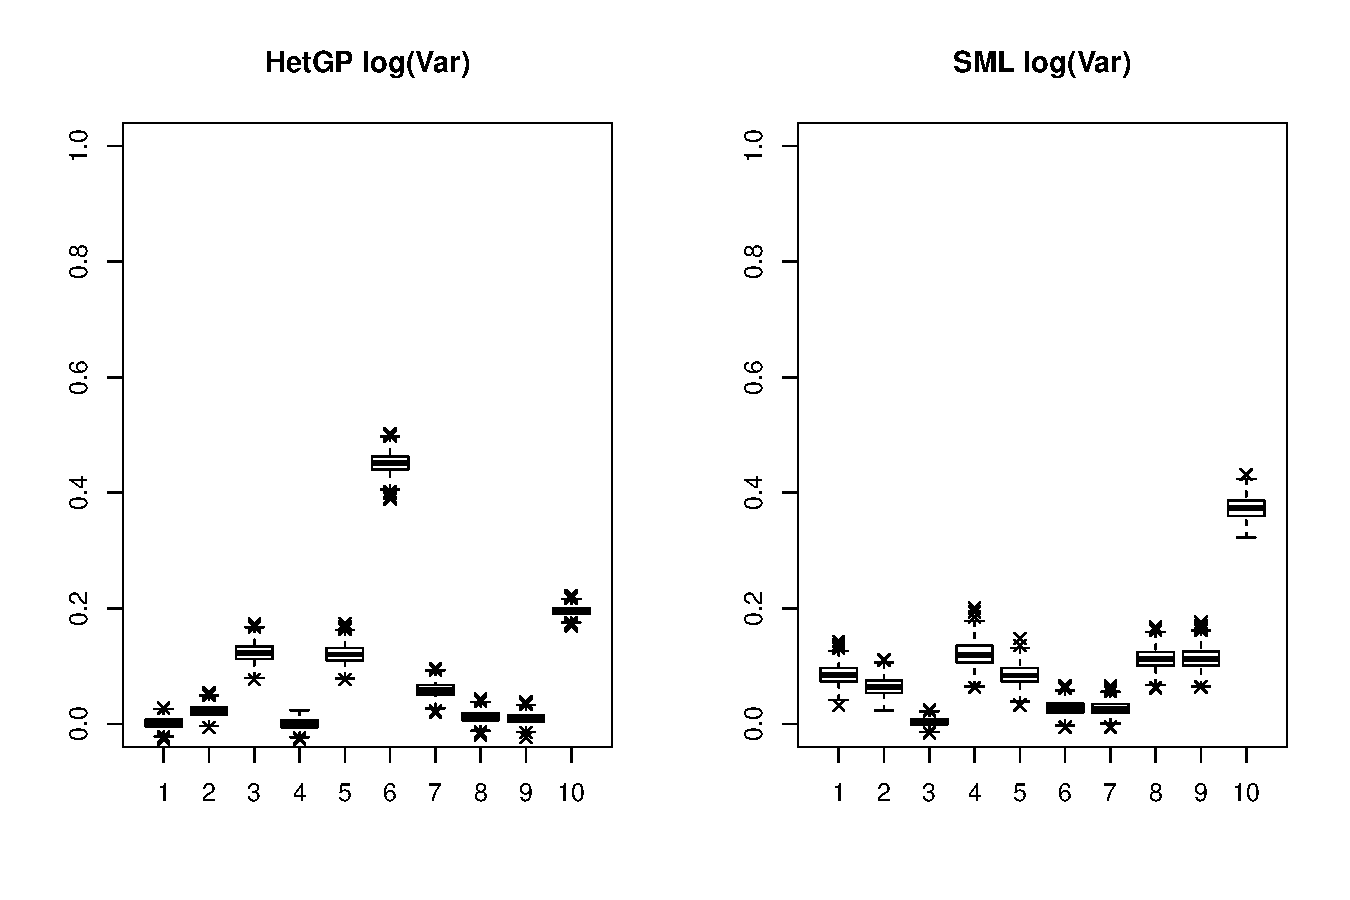
\includegraphics[width=0.9\textwidth]{fig-sensitivity/si-var4.pdf}
  \caption{Boxplots representing the posterior distribution of $S_i^{\lambda}$; $i=1$, $2$, \ldots, $9$. The $10^{th}$ index corresponds to $S_{T_\varepsilon}$. Left hand plot corresponds to HetGP; right hand to SML.}
   \label{Fig:si-var}
\end{figure}
\begin{figure}[ht]
   \centering
   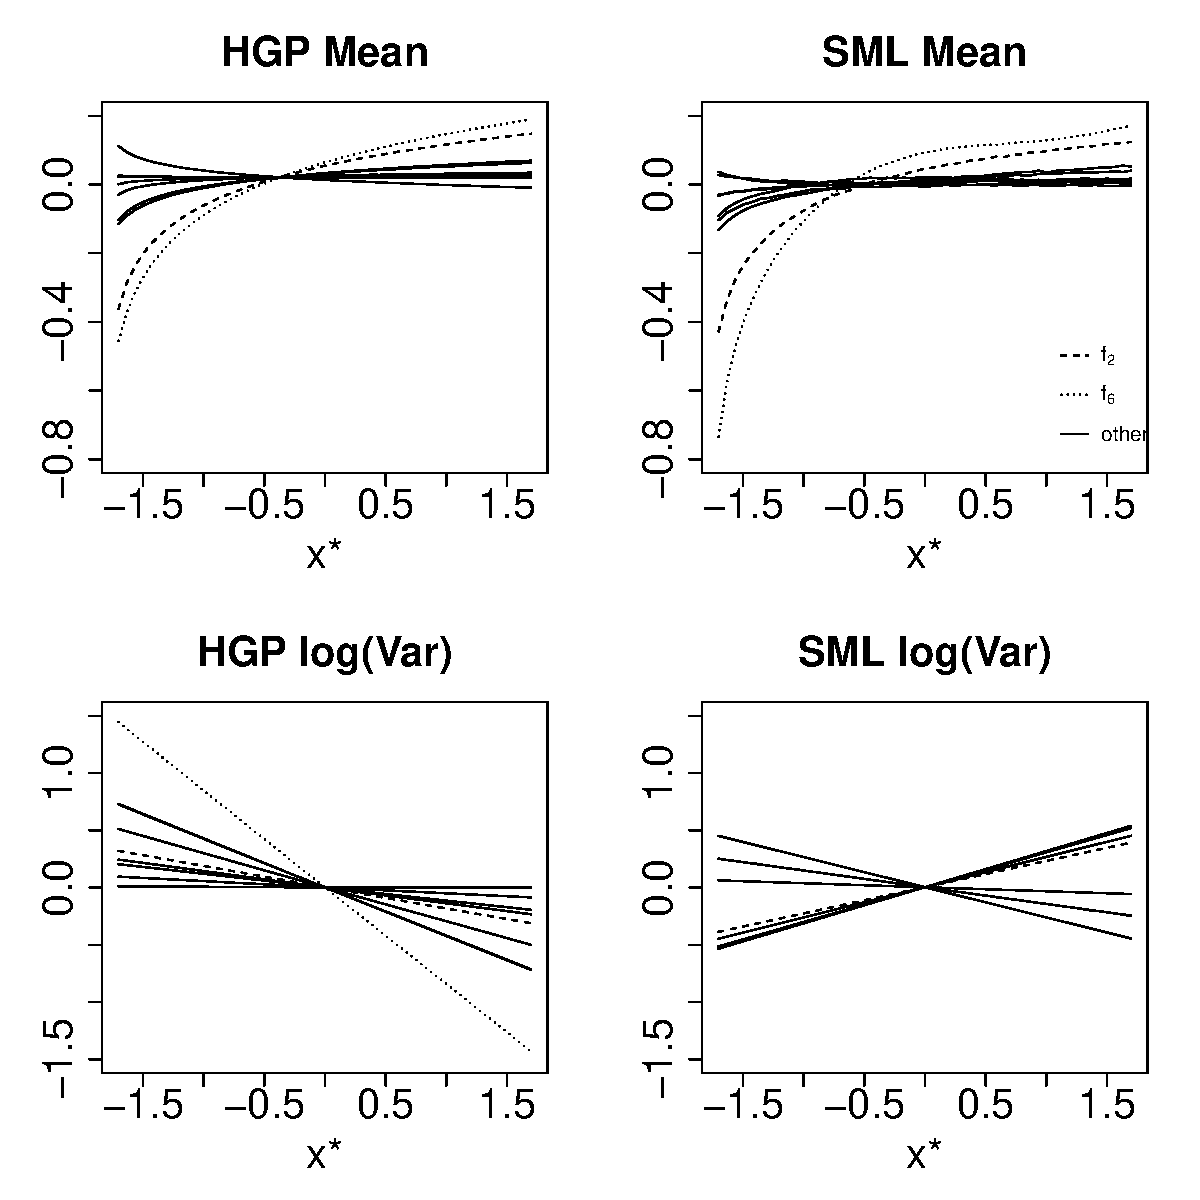
\includegraphics[width=0.9\textwidth]{fig-sensitivity/main-effects-all.pdf}
     \caption{Main effect plots under HetGP (left) and SML (right). Top plots correspond to the mean surface and bottom plots to the log variance surface. The dashed lines correspond to $f_2(x_2)$ and $f_2^{\lambda}(x_2)$, dotted lines to $f_6(x_6)$ and $f_6^{\lambda}(x_6)$. The solid lines represent all other main effects. The $x$ axis is on the standardised scale that the emulators were fitted on. Note that the scale of the $y$ axis on the mean plot differs from that of the variance plot.}
  \label{Fig:main-eff-all}
\end{figure}

We see that qualitatively, the plots of main effects (\Cref{Fig:main-eff-all}) agree with the estimated values of $S_i$ and $S^{\lambda}_i$. That is, an input with high $S_i$ exhibits a large range in the main effect plot. The main effect plots for the mean are quite similar with the exception of $f_6(x_6)$. Under SML $f_6(x_6)$ has a much larger range and the shape of $f_6(x_6)$ is different under the two approaches. The HetGP estimate looks very close to $\log(x_6)$; the chosen mean function. This suggests that SML is borrowing information from the cheap simulator to inform the mean response of the expensive simulator and marries up with the (lack of) structure in the residual plots seen earlier (\Cref{Fig:het-resids}, \Cref{Fig:sml-resids}). The main effects for the log variance are quite different under the two emulators. Under HetGP, $x_6$ is highly influential for the log variance, whereas $x_6$ is much less influential under the SML emulator. A stark difference is that the slopes of many of the $f_{i}^{ \lambda }(x_i)$ are of opposite sign under the two emulators. For example, the slope of $f_2^{ \lambda }(x_2)$ under SML is positive which matches up with empirical estimates given in \Cref{Fig:log-vars}.  We believe this is due to SML resolving a kind of weak identifiability issue; when insufficient data is fed to a HetGP emulator, systematic variation can be interpreted as noise. \cref{Fig:log-vars} shows logged sample estimates $\var \{ y(\bx) \} $. Namely, we have plotted $\log s^2(\bx)$ where
\begin{equation}
  s^2(\bx) =  \frac{1}{N-1} \sum_{i = 1}^N \left\{\probit[A(\bx)]_i - \overline{\probit}[A(\bx)]\right\}^2
\end{equation}
is the (estimated) variance of the probit availability, and availability is defined at the mean point-wise availability over the first $5$ years of the wind farm's life time. The $i$ subscript is used to denote replicates at the same value of $\bx$. The \correction{data plotted in \cref{Fig:log-vars} are based} on a round of simulations independent of training data of any emulators. We only varied $x_2$ to construct this plot. Although we were critical of OAT analyses earlier, we can justify fixing the other inputs here as our sensitivity analysis showed the interaction terms were negligible thus varying inputs one-at-a-time is a reasonable way to sense-check the main effect plots.

\begin{figure}
  \centering
  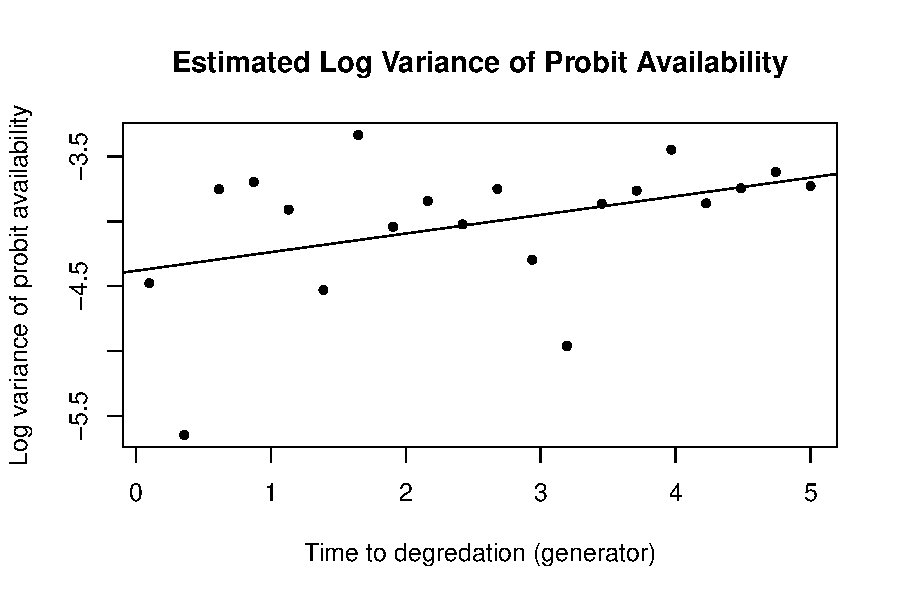
\includegraphics[width = 6in]{sml-het-fig2/log-var-reps2.pdf}
  \caption{Log sample variances of $\probit[A(\bx)]$ at equally spaced points on $[0.1, 5]$. Each estimate is based on $10$ replicates of the expensive version of Athena considered in \cref{Ch:Hetsml} and generated independently of any emulator training data. \label{Fig:log-vars}}
\end{figure}
\section{Conclusions}
We have now performed the necessary analyses to set up a future elicitation procedure. Using the results from either the SML or HetGP emulators the largest contributions to output uncertainty were the failures of the blades ($x_6$) and generator ($x_2$). An equi-tailed $95\%$ credible interval (computed via SML) for $S_2 + S_6$ is $(59,73)\%$ of input uncertainty. Note that this estimate does not include $S_{2,6}$, the contribution of uncertainty due to the interaction between $x_2$ and $x_6$. The simulator appears to be approximately additive, thus $S_{2,6} \approx 0$. The results of the sensitivity analysis were also used to help understand why one of two competing emulators performed worse than the other. A second round of elicitation of $\bx$ would focus mainly on the lifetime parameters of the generator ($x_2$) and the turbine blades ($x_6$), since they jointly contribute to over half of output uncertainty. The other inputs would not be completely neglected since they contribute roughly equal amounts of uncertainty to the log variance. Without an emulator this sensitivity analysis would have taken many months of CPU time. Our SML emulator allowed us to further reduce the amount of time required to construct an adequate emulator by exploiting a computationally cheaper version of the Athena simulator.

One issue that we have not explored here is understanding which input(s) have the largest overall impact on $y(\bx)$. Suppose that, for an $m$ dimensional simulator, the largest $S_i$ is $S_1$ and the smallest is $S_m$. Further suppose that $S^{\lambda}_1$ is the \textit{smallest} sensitivity index for the log variance and $S^{\lambda}_m$ is the \textit{largest}. In such a scenario it is not clear whether $x_1$ is more or less important than $x_m$. In a deterministic setting, if we know the precise value of $\bx$ then we can find $f(\bx)$. In the stochastic case, knowing $\bx$ means we can find the distribution of $y(\bx)$. One way to do this would be to formulate a utility function $U(\bx) = \tilde{U} ( y(\bx))$ and perform an EVPI analysis, on $U(\bx)$. $U(\bx)$ should reflect which aspects of $y(\bx)$ are most critical to our application. For example, if our aim is to find input settings which lead to the average availability, $A(\bx)$, being above some threshold $A^{*}$ then $u(\bx) = \mathbb{I}(A(\bx) > A^{*})$ would be an appropriate utility function (remembering that $\E\{u(\bx)\}  = U(\bx)$). This would be equivalent to emulating, and performing an EVPI analysis on $\Pr (A(\bx) >  A^{*})$.

If the analysis is concerned with understanding which inputs are driving the entire distribution (rather than a single summary), it may be advantageous to borrow ideas from the Bayesian design of experiments literature. In Bayesian design of experiments, one will have a prior specification for the parameters of a statistical model, and the design should aim to maximise a summary of the posterior, such as some notion of difference between prior and posterior \citep{Prangle2022}. A concrete idea would be to construct a HetGP emulator for $y(\cdot)$ then use Kullback-Leibler divergence as a utility function within an EVPI framework. Since, under GP assumptions, $y(\bx)\mid\bx \sim N(\mu(\bx),\lambda^2(\bx))$ we may be able to obtain a tractable analysis by assuming $y(\bx) \sim \mathcal{N}(M, V)$. In particular, if $\bx'$ is a known simulator input, then assuming $y(\bx)$ and $y(\bx')$ are Normally distributed we have
\begin{equation}
  U(\bx') = \text{KL}(y(\bx') || y(\bx)) = \log \left( \frac{\hat{\lambda}(\bx')}{\sqrt{V}} \right) + \frac{\hat{\lambda}^2(\bx') + (m^{*}(\bx') - M)^2}{2V} - \frac{1}{2}.
\end{equation}
Then, by an EVPI analysis, the input $i$ with largest EVPI would be the most influential input on the distribution of $y(\cdot)$. Since, with an emulator, $m^{*}$ and $\lambda^2(\bx)$ are quick to compute, this analysis should be tractable within a frequentist framework or an Empirical Bayes framework like the emulators described in \cref{Ch:Hetsml}. A fully Bayesian equivalent to the analysis would have to average over $\pi \{ y(\cdot) \mid \mathcal{D} \}$. This is similar to the approach taken by \citet{Oakley2009}, who performs an EVPI analysis, assisted by emulators, to deduce which of three medical treatments offers the most viable solution. EVPI analysis comes into play as a way to check the robustness of the optimal decision. This is perhaps more useful than performing PSA on the mean and log variance separately. Of course, performing PSA on the mean and variance has many valid use cases. It allows us to investigate the behaviour of a complex, black-box stochastic simulator. We used the results of PSA to diagnose potential issues with an emulator We used the fact that the main effect plots of the log variance generated by HetGP were inconsistent with our knowledge of Athena to understand that the HetGP emulator was confusing systematic and random variation. In other words, we extended this idea to \textit{emulator} validation. On a similar vein, \citet{Kennedy2006} used the main effect plots to verify that a vegetation model produced sensible outputs. The outputs were deemed unusual which led to the discovery of a bug in the simulator under study.
\end{chapter}
